\section{Results}
\label{sec:results}

\begin{table}[t]
\caption{Main comparison on the 112-case benchmark (Qwen2.5-7B-Instruct, $r=0.50$, seed
20261015). All arms of ours are constructed without access to the reference answer.
\emph{tokens} is the mean compressed-context length; \emph{leak} counts cases in which a
protected value is recoverable from question plus context. Arrows give the preferred
direction. $BCL$ $=$ \arm{budget\_cluster\_link}, $ABL$ $=$ \arm{alias\_budget\_link},
$ALB$ $=$ \arm{alias\_budget}, $BC$ $=$ \arm{budget\_cluster}. Controlled comparison is the
first three rows: compressing to $48.6\%$ of the original length costs $0.0109$ against the
no-compression aliasing arm, which is not significant. The uncompressed arm is the reference
value used to verify that a result set belongs to this benchmark.}
\label{tab:main}
\centering\small
\setlength{\tabcolsep}{3pt}
\begin{tabular}{lrrr}
\toprule
Arm & F1 $\uparrow$ & tokens $\downarrow$ & leak $\downarrow$ \\
\midrule
\arm{full}                 & 0.7189 & 7964 & 112/112 \\
\arm{alias}                & 0.6475 & 7824 & 0/112 \\
\textbf{\textsc{DARK}} & \textbf{0.6366} & \textbf{3869} & \textbf{0/112} \\
\arm{delete}               & 0.4916 & 7845 & 0/112 \\
BCL                        & 0.4308 & 3683 & 47/112 \\
ABL                        & 0.4219 & 3638 & 0/112 \\
ALB                        & 0.2232 & --- & 0/112 \\
BC                         & 0.2143 & --- & 8/112 \\
\bottomrule
\end{tabular}
\begin{tablenotes}\footnotesize
\item[] Paired differences against \textsc{DARK}: \arm{alias} $-0.0109$
$[-0.0824,+0.0612]$ (n.s.); \arm{full} $-0.0823$ $[-0.1610,-0.0041]$;
ABL $+0.2147$ $[+0.1224,+0.3085]$.
\end{tablenotes}
\end{table}


\subsection{Compression costs little}

Table~\ref{tab:main} answers the first question: at an equal $50\%$ budget, does the routing
rule preserve the task? Aliasing the whole context without compressing scores $0.6475$;
\textsc{DARK} scores $0.6366$ at $48.6\%$ of the tokens. The paired difference is
$-0.0109$ with a $95\%$ interval of $[-0.0824,+0.0612]$, which does not exclude zero: on
this benchmark, halving the context costs no measurable task quality relative to the
leak-free uncompressed arm. Against not compressing and not sanitizing, the deficit is
$-0.0823$ $[-0.1610,-0.0041]$, which is the price of the privacy constraint rather than of
compression, since the aliasing arm pays it as well ($-0.0714$ against \arm{full}).

The comparison specific to our design is the lower block of the table. Two arms are
leak-free and compress to nearly the same length: \arm{alias\_budget\_link}, which aliases
globally and protects the anchor line, and \textsc{DARK}. The difference is $+0.2147$
$[+0.1224,+0.3085]$. The two do not differ in the privacy operation---both alias---but in
which region survives: one line, or the block containing it.

\begin{table*}[t]
\caption{Comparison on the 2{,}728-case extension (Qwen2.5-7B-Instruct, $r=0.50$). Published
compressors are re-run through their reference implementations on the same cases; arms
suffixed \arm{\_native} use each method's own default length. \emph{Leak} is the fraction of
cases in which a protected value is recoverable from the prompt. \textsc{DARK} and the
masking baseline are the only arms at $0\%$; \textsc{DARK} exceeds that baseline by
$+0.3226$ $[+0.3041,+0.3414]$. Against the strongest compressor, Quito-X, the difference is
$+0.0107$ $[-0.0091,+0.0306]$, i.e.\ not significant, at $0\%$ versus $98.1\%$ leakage.
The uncompressed arm reproduces the reference value $0.6078$ from a separately evaluated
batch to within one case in $2{,}728$.}
\label{tab:external}
\centering\small
\setlength{\tabcolsep}{6pt}
\begin{tabular}{llrr}
\toprule
Method & Family & F1 $\uparrow$ & leak $\downarrow$ \\
\midrule
\arm{full}                     & uncompressed       & 0.6081 & 100.0\% \\
\arm{ext\_full}                & uncompressed (rerun) & 0.6078 & 100.0\% \\
\textbf{\textsc{DARK}}     & ours (routes)      & \textbf{0.4937} & \textbf{0.0\%} \\
Quito-X                        & query-aware        & 0.4831 & 98.1\% \\
Quito-X \arm{\_native}         & query-aware        & 0.4862 & 98.1\% \\
CPC                            & query-aware        & 0.4740 & 92.6\% \\
CPC \arm{\_native}             & query-aware        & 0.4523 & 93.4\% \\
Provence                       & query-aware        & 0.4080 & 90.8\% \\
Provence \arm{\_native}        & query-aware        & 0.4047 & 88.8\% \\
\arm{alias\_budget\_link}      & ours, no answer key, merged cell & 0.3482 & 0.0\% \\
\arm{budget\_cluster\_link}    & raw text, anchor kept & 0.3352 & 55.4\% \\
\arm{quad4\_del}               & ours, delete instead of alias & 0.3142 & 0.0\% \\
LLMLingua-2                    & task-agnostic      & 0.2651 & 100.0\% \\
LLMLingua-2 \arm{\_native}     & task-agnostic      & 0.2433 & 100.0\% \\
\arm{mask\_llmlingua2}         & sanitize + compress & 0.1712 & 0.0\% \\
\arm{mask\_llmlingua2\_native} & sanitize + compress & 0.1663 & 0.0\% \\
\arm{alias\_budget}            & global alias, no anchor & 0.1469 & 0.0\% \\
\arm{budget\_cluster}          & redundancy only    & 0.0981 & 0.5\% \\
\bottomrule
\end{tabular}
\end{table*}


\subsection{At scale, the comparison is a privacy comparison}

Table~\ref{tab:external} reports the $2{,}728$-case extension. \textsc{DARK} scores
$0.4937$, level with the strongest query-aware compressor (Quito-X, $0.4831$; difference
$+0.0107$, interval $[-0.0091,+0.0306]$) and above CPC ($0.4740$) and Provence ($0.4080$).
What separates the arms is leakage. Every published compressor leaves protected values in
the prompt, in $88.8\%$ to $100\%$ of cases, because concealing them is not among its
objectives. \textsc{DARK} leaves none. Among leak-free arms the nearest competitor is a
masking wrapper at $0.1712$, which \textsc{DARK} exceeds by $+0.3226$
$[+0.3041,+0.3414]$.

The reading we take from this table is narrow. A query-aware compressor reaches the same F1
as our rule at the same budget, but only by forwarding the value the question names. When
that value must not be forwarded, the compressor loses the task, as the masking row shows,
and the routing rule does not.

\begin{table}[t]
\caption{Budget curve on the 112-case benchmark. Every row satisfies its budget with zero
overshoot. \textsc{DARK} is the strongest budget arm at all five ratios; its advantage
narrows as the budget grows, and its own score peaks at $r=0.50$ because at $r=0.75$ the
additional refill text is noise. The last row gives the mean realised context length in tokens.}
\label{tab:budget}
\centering\small
\setlength{\tabcolsep}{3pt}
\resizebox{\columnwidth}{!}{%
\begin{tabular}{lrrrrr}
\toprule
Arm & @0.10 & @0.15 & @0.25 & @0.50 & @0.75 \\
\midrule
\textbf{\textsc{DARK}} & \textbf{0.4357} & \textbf{0.4681} & \textbf{0.5116} & \textbf{0.6366} & \textbf{0.6158} \\
\arm{quad4\_del}           & 0.3297 & 0.3788 & 0.3955 & 0.5205 & 0.5086 \\
BCL                        & 0.2304 & 0.2052 & 0.2310 & 0.4308 & 0.5576 \\
ABL                        & 0.2304 & 0.2052 & 0.2488 & 0.4219 & 0.5512 \\
\midrule
realised tokens            & 656 & 1033 & 1913 & 3869 & 5830 \\
\bottomrule
\end{tabular}}
\vspace{2pt}
{\footnotesize Uncompressed reference: F1 $0.7189$ at $7964$ tokens.}
\end{table}


\begin{figure*}[t]
\centering
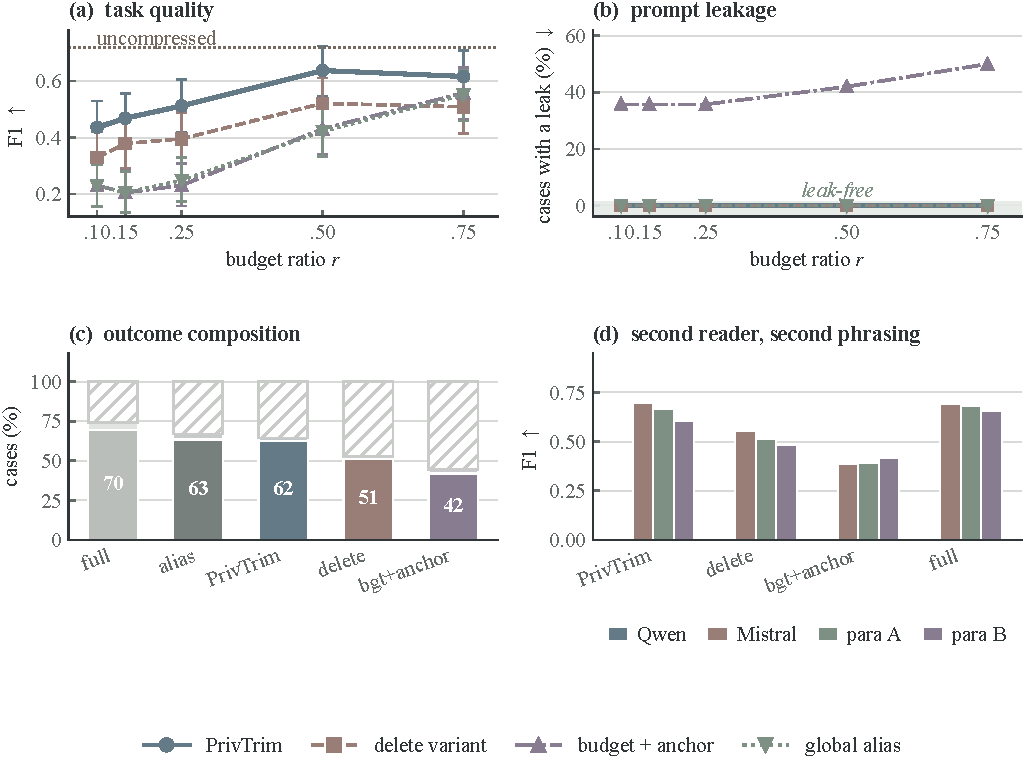
\includegraphics[width=\textwidth]{figures/fig1_main.pdf}
\caption{Behaviour across the budget sweep (112 cases). (a) F1 at five ratios with bootstrap
$95\%$ intervals over cases; the dotted line is the uncompressed reference. (b) Fraction of
cases in which a protected value is recoverable from the prompt. \textsc{DARK}, the
delete variant and the global-alias arm stay at zero for the whole range, while the arm that
compresses raw text leaks in $35.7\%$ of cases at tight budgets and $50.0\%$ at $r=0.75$, so
its apparent parity at loose budgets is bought with exposure. (c) Composition of case
outcomes at $r=0.50$: solid is an exact answer, the pale band is a partial match, hatched is
a wrong or \textsc{unknown} answer. (d) The same four arms under a second reader and two
question paraphrases; the ordering of the arms is preserved in all four conditions.}
\label{fig:budget}
\end{figure*}

\subsection{The advantage holds across budgets}

Table~\ref{tab:budget} varies the budget over five ratios. \textsc{DARK} is the strongest
budget arm at every point: $+0.205$ at $r=0.10$, $+0.263$ at $r=0.25$, $+0.215$ at
$r=0.50$, and $+0.065$ at $r=0.75$, all at zero leakage. Its own score is not monotone. It
peaks at $r=0.50$ and drops by $0.021$ at $r=0.75$, because the additional refill text admitted
at a loose budget is repetitive context that competes with the relevant block for the
reader's attention. The competing arms keep improving with budget, so the margin narrows;
at $r=0.75$ it is small. We report the non-monotonicity rather than describing the curve as
monotone, and note that the half-budget setting used elsewhere is where the mechanism
separates most clearly from the alternatives.

\subsection{Cross-model and phrasing stability}

On Mistral-7B-Instruct-v0.3 at $r=0.50$, \textsc{DARK} scores $0.6946$ against $0.6366$
on Qwen2.5-7B. Every other arm loses ground when the reader changes: \arm{full} $-0.0258$,
\arm{alias} $-0.0544$, \arm{delete} $-0.0357$, \arm{alias\_budget\_link} $-0.0471$,
\arm{budget\_cluster\_link} $-0.0471$. The routing rule is the only arm that improves, which
is consistent with the mechanism: a second reader gains more from a cleaned, budgeted prompt
than from a long one.

Against two mechanical rewritings of the question, \textsc{DARK} scores $0.6637$ and
$0.6023$ against $0.6366$ on the original, a maximum change of $-0.0343$. The uncompressed
arm changes by $-0.0614$ over the same rewritings. The margin over
\arm{alias\_budget\_link} remains significant in all three conditions ($+0.2147$, $+0.2711$,
$+0.1994$). The check is relevant because the rule keys on a mention of the queried entity,
and a rewriting could in principle disturb that mention; in these variants it does not.
